\documentclass[11pt]{beamer}
\usetheme{Madrid}
\usecolortheme{dolphin}
\usepackage[utf8]{inputenc}
\usepackage[T1]{fontenc}
\usepackage{amsmath,amssymb,amsthm}
\usepackage{graphicx}
\usepackage{booktabs}
\usepackage{siunitx}
\usepackage{comment}
% \usepackage[hidelinks]{hyperref}

% Title
\title[Synthetic turbulent field]{Synthetic turbulence generation using
statistical methods}
\author[Samy Braik]{Samy Braik \\[0.5em] \small Supervisor: Aurélien Larcher\inst{1}, Jonathan Viquerat\inst{1}, Fabien Duval\inst{2} and Aubin Brunel\inst{2}}
\institute{
  \inst{1}CEMEF, Mines Paris–PSL \\
  \inst{2}ASNR
}\date{\today}

\begin{document}

\begin{frame}
  \titlepage
  % \includegraphics[options]{illustrations/M}
\end{frame}

\begin{comment}
\begin{frame}{Outline}
  \tableofcontents
\end{frame}
\end{comment}

\section{Introduction}
\begin{frame}{What is turbulence?}
  \begin{itemize}
    \item Turbulence: complex, aperiodic fluid motion with strong vortical structures.
    %\item Contrasts with laminar flow; typically characterized by high Reynolds number $\mathrm{Re}$.
    \item We study \emph{Homogeneous and Isotropic Turbulence (HIT)}: statistics invariant under space translations and rotations.
  \end{itemize}
  \vfill
  \begin{figure}
    \centering
    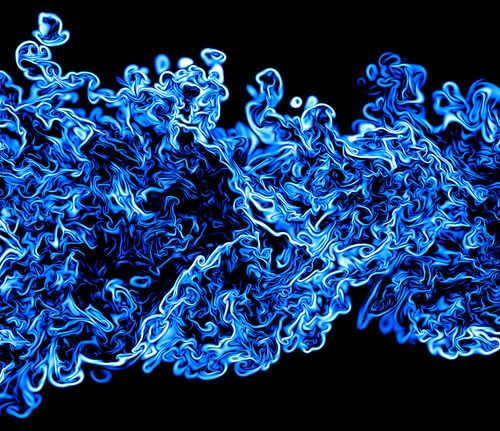
\includegraphics[width=0.5\textwidth]{illustrations/TurbulenceExample.jpg}
    \caption{Slice through scalar dissipation (CNRS UMR 6614 CORIA and JSC).}
  \end{figure}
\end{frame}

\section{Model}

\subsection{Random Fourier model}
\begin{frame}{Random Fourier model}
  \begin{itemize}
    \item Build a synthetic velocity field by summing random Fourier modes.
    \item Frozen-turbulence assumption (no time dependence):
  \end{itemize}
  \begin{equation}
    u^s(x)= 2\sum_{n=1}^{N} \hat{u}_n \cos(\kappa^n\cdot x + \psi_n)\,\sigma^n
  \end{equation}
  \begin{description}
    \item[$\kappa^n$] wave vector (random on a half-sphere to preserve isotropy)
    \item[$\sigma^n$] direction (divergence-free: $\kappa^n\cdot\sigma^n=0$)
    \item[$\psi_n$] random phase (uniform $\mathcal{U}[0,2\pi]$)
    \item[$\hat{u}_n$] amplitude linked to prescribed energy spectrum $E(\kappa_n)$
  \end{description}
\end{frame}

\begin{frame}{Coefficient sampling}
  \begin{itemize}
    \item Wave vector components (spherical coordinates):
        \begin{align}
            \kappa_1 &= \sin(\theta)\cos(\varphi) \\
            \kappa_2 &= \sin(\theta)\sin(\varphi) \\
            \kappa_2 & = \cos(\theta)
        \end{align}
    \item Sampling densities: $f_\theta(\theta)=\frac{\sin\theta}{2}$, $f_\varphi(\varphi)=\frac{1}{2\pi}$.
    \item Direction vector $\sigma$ obtained by fixing an angle $\alpha\sim\mathcal{U}[0,2\pi]$ and ensuring $\kappa\cdot\sigma=0$.
        \begin{align}
            \sigma_1&=\cos(\varphi)\cos(\theta)\cos(\alpha)-\sin(\varphi)\sin(\alpha) \\
            \sigma_2&=\sin(\varphi)\cos(\theta)\cos(\alpha)+\cos(\theta)\sin(\alpha) \\
            \sigma_3&=-\sin(\theta)\cos(\alpha)
        \end{align}
  \end{itemize}
\end{frame}

\begin{frame}
  \begin{figure}
    \centering
    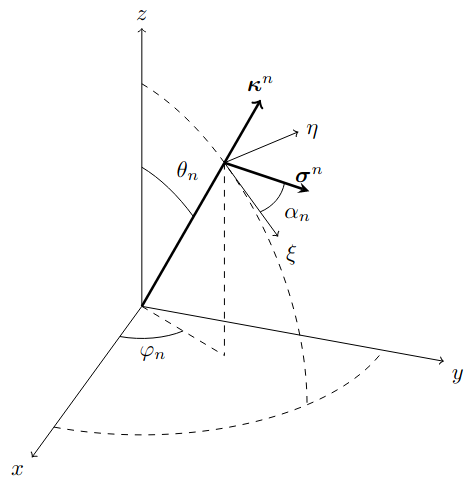
\includegraphics[width=0.6\linewidth]{illustrations/WaveVectorGeometry.png}
    \caption{Wave vector geometry}
  \end{figure}
\end{frame}

\subsection{Energy spectrum}
\begin{frame}{Energy spectrum}
  \begin{itemize}
    \item von K\'arm\'an–Pao (VKP) energy spectrum: $E_{\mathrm{VKP}}(\kappa)=\frac{2}{3}\alpha_e\,\kappa L_e\frac{(\kappa L_e)^4}{[(\kappa L_e)^2+1]^{17/6}}\exp\big(-2(\kappa L_\eta)^2\big)$ 
  \end{itemize}
  \begin{figure}
    \centering
    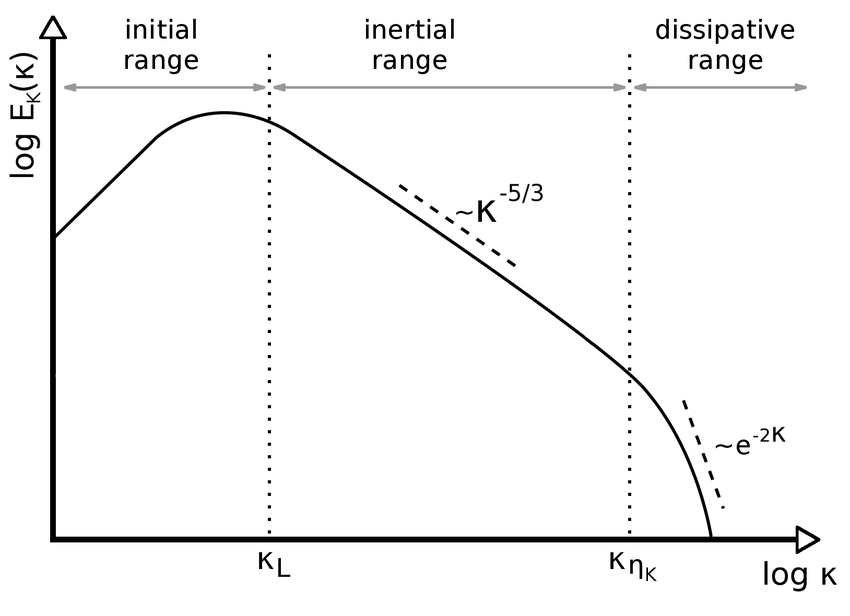
\includegraphics[width=0.7\linewidth]{illustrations/energy-spectrum-example.png}
    \caption{Energy spectrum of a turbulent flow}
  \end{figure}
\end{frame}

\begin{comment}
\begin{frame}
  \begin{itemize}
  \item To capture large- and small-scale behavior use a full model such as von K\'arm\'an–Pao (VKP):
      \begin{equation}
        E_{\mathrm{VKP}}(\kappa)=\frac{2}{3}\alpha_e\,\kappa L_e\frac{(\kappa L_e)^4}{[(\kappa L_e)^2+1]^{17/6}}\exp\big(-2(\kappa L_\eta)^2\big)
      \end{equation}
    \item Mode amplitudes: $\hat{u}_n=\sqrt{E(\kappa_n)\,\Delta\kappa_n}$ (log-spacing used for $\kappa_n$).
  \end{itemize}
  \begin{figure}
    \centering
    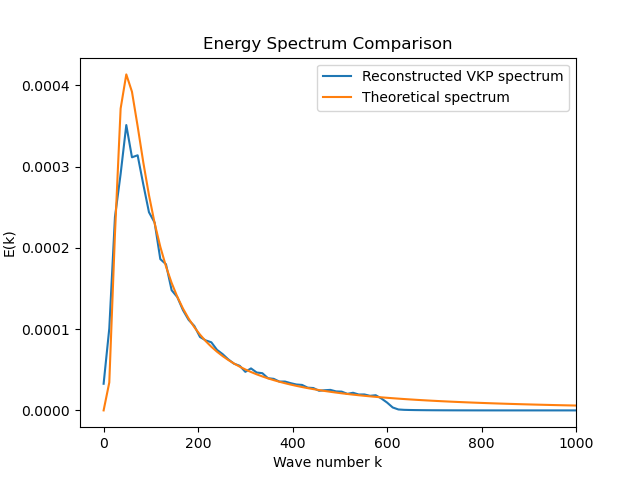
\includegraphics[width=0.59\textwidth]{illustrations/Energy_Spectrum_VKP.png}
    \caption{VKP spectrum vs theoretical reference}
  \end{figure}
\end{frame}
\end{comment}

\begin{comment}
\section{Metrics \& Limitations}
\begin{frame}{Metrics to assess synthetic field}
  \begin{itemize}
    \item Energy spectrum reconstruction: match between theoretical and reconstructed $E(\kappa)$.
    \item Component means close to zero (homogeneity).
    \item RMS speed must match prescribed value.
    \item Velocity increments statistics (non-Gaussian heavy tails expected at small scales).
  \end{itemize}
\end{frame}

\begin{frame}{Parameters used}
  \begin{center}
  \begin{tabular}{lll}
  \toprule
  \textbf{Parameter} & \textbf{Value} & \textbf{Unit}\\
  \midrule
  Number of points & $100^3$ & --\\
  Length of box & $\tfrac{\pi}{6}$ & \si{\meter}\\
  Number of modes & 500 & --\\
  RMS speed & 0.222 & \si{\meter\per\second}\\
  Integral length scale & 0.024 & \si{\meter}\\
  Viscosity & $1.8\times10^{-5}$ & \si{\meter^2\per\second}\\
  Minimum wave number & $\tfrac{2\pi}{1.0}$ & \si{\per\meter}\\
  Maximum wave number & $\tfrac{2\pi}{0.01}$ & \si{\per\meter}\\
  \bottomrule
  \end{tabular}
  \end{center}
\end{frame}

\begin{frame}{Empirical base metrics}
  \begin{table}
    \centering
    \begin{tabular}{lr}
      \toprule
      \textbf{Direction} & \textbf{Mean} \\
      \midrule
      x & -0.00269 \\
      y & -0.00010 \\
      z & -0.00126 \\
      \bottomrule
    \end{tabular}
    \qquad
    \begin{tabular}{lr}
      \toprule
      \textbf{Direction} & \textbf{RMS (expected: 0.222)} \\
      \midrule
      x & 0.19583 \\
      y & 0.17599 \\
      z & 0.19307 \\
      \bottomrule
    \end{tabular}
    \caption{Velocity mean and RMS}
  \end{table}
\end{frame}

\begin{frame}{Velocity increments \& heavy tails}
  \begin{itemize}
    \item Velocity increments: $\delta_r u = u(x+r)-u(x)$.
    \item In random Fourier base model increments are typically Gaussian (kurtosis $=3$).
    \item Real turbulence: increments show heavy tails (increasing kurtosis when $r\to 0$).
  \end{itemize}
  \begin{figure}
    \centering
    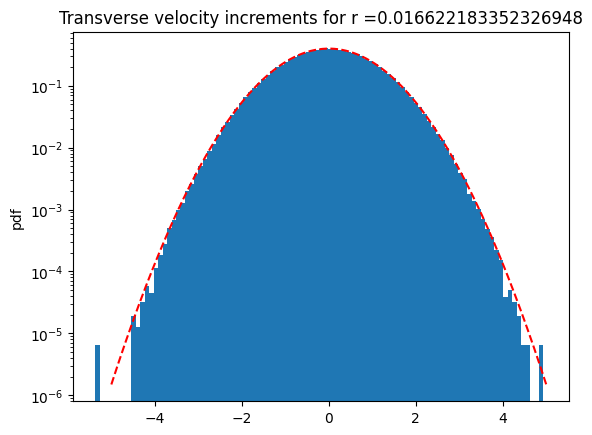
\includegraphics[width=0.45\textwidth]{illustrations/TransVelIncrExample.png}
    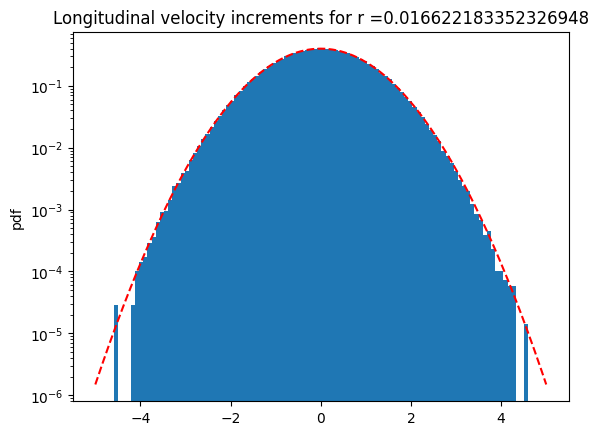
\includegraphics[width=0.45\textwidth]{illustrations/LongVelIncrExample.png}
    \caption{Transverse and longitudinal increments (model vs Gaussian)}
  \end{figure}
\end{frame}

\begin{frame}{Random Fourier Velocity field}
  \begin{figure}
    \centering
    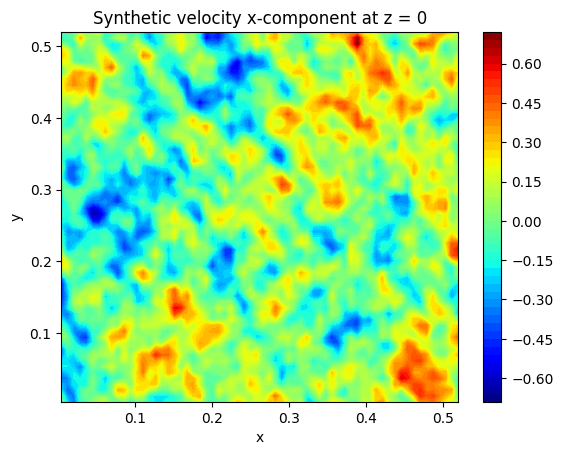
\includegraphics[width=0.6\textwidth]{illustrations/Velocity_Example.png}
    \caption{Synthetic velocity field obtain via random Fourier model}
  \end{figure}
\end{frame}

\section{Method}
\begin{frame}{Goal and strategy}
  \begin{itemize}
    \item \textbf{Goal:} produce heavy-tailed velocity increments while preserving energy spectrum and isotropy.
    \item \textbf{Strategy:} parameterize coefficients (angles, phases, amplitudes) as learnable parameters (\texttt{nn.Parameter} in PyTorch) and optimize a loss using AdamW(lr=1e-3).
  \end{itemize}
\end{frame}
\end{comment}

\begin{comment}
\begin{frame}{Losses}
  \begin{block}{Flatness (excess kurtosis) objective}
    \begin{itemize}
      \item Use flatness (= kurtosis $-$ 3) of velocity increments as a loss term to encourage heavy tails.
      \begin{align}
        \mathcal{L}_F = \frac{1}{n}\sum_{i=1}^{n}(kurt-3-F_\text{target})
      \end{align}
    \end{itemize}
  \end{block}
  \begin{block}{Energy-spectrum objective}
    \begin{itemize}
      \item MSE between reconstructed and target spectrum, optionally with a smoothness regulariser (penalize high-frequency oscillations in $E(\kappa)$).
      \begin{align}
        L_{ES} = \frac{1}{n}\sum_{i=1}^{n}(E_{\text{rec},i}-E_{\text{theory},i})^2
      \end{align}
    \end{itemize}
  \end{block}
  \vfill
  \centering Combined loss: $\mathcal{L}=\mathcal{L}_F + 10^3\mathcal{L}_{ES}$
\end{frame}


\subsection{Preliminary experiments}
\begin{frame}{Preliminary experiments}
  \begin{itemize}
    \item Tested optimization toward Gaussian target flatness (flatness $=0$) from different initialization.
    \item Starting from Gaussian increments: parameters remain close to initial Janin et al. choice.
    \item Starting from heavy-tailed increments: $\theta$ adapt to a flatter distribution.
  \end{itemize}
  \begin{figure}
    \centering
    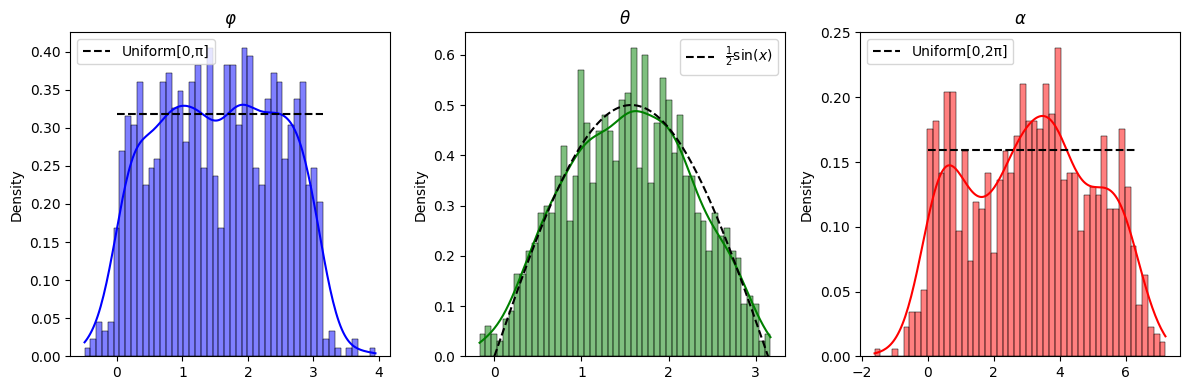
\includegraphics[width=0.9\textwidth]{illustrations/StartGaussian.png}
    \caption{Angle distributions starting from Gaussian increments}
  \end{figure}
\end{frame}


\begin{frame}{Preliminary experiments}
  \begin{figure}
    \centering
    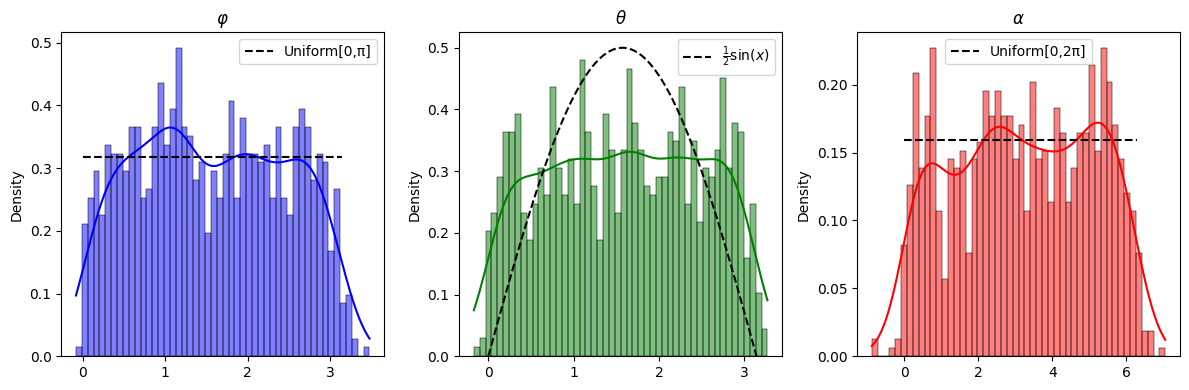
\includegraphics[width=0.9\textwidth]{illustrations/StartHeavyTail.png}
    \caption{Angle distributions starting from heavy-tailed increments}
  \end{figure}
  \begin{itemize}
    \item Observations: RMS and means largely preserved while increment statistics change.
  \end{itemize}
\end{frame}
\subsection{First approach}
\begin{frame}{First approach}
  \begin{itemize}
    \item Work on $(\psi,\kappa,\sigma)$
  \end{itemize}
  \begin{figure}
    \centering
    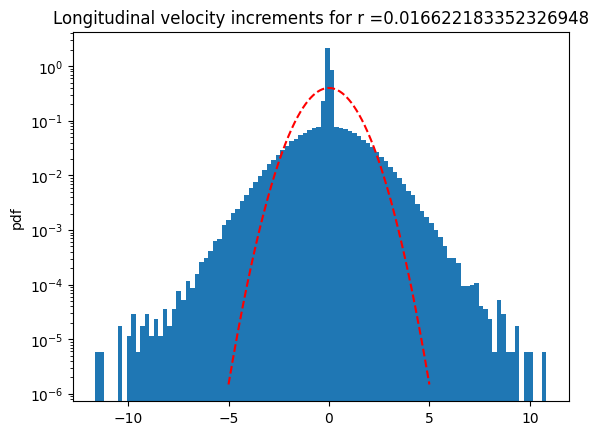
\includegraphics[width=0.45\textwidth]{VelIncrPSIKAPPASIGMA/VelIncrLong.png}
    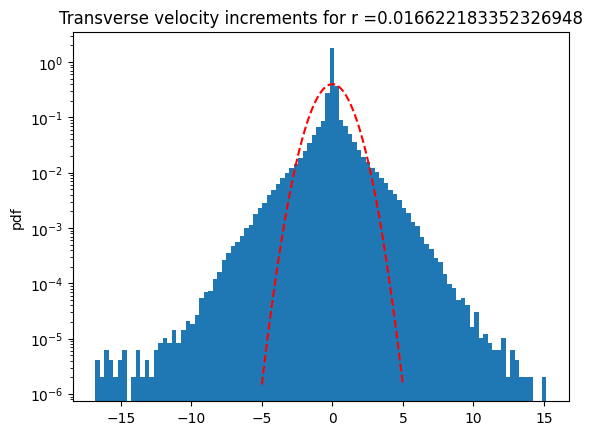
\includegraphics[width=0.45\textwidth]{VelIncrPSIKAPPASIGMA/VelIncrTrans.png}
    \caption{Velocity increments after learning on $(\psi,\kappa,\sigma)$}
  \end{figure}
\end{frame}

\begin{frame}
  \begin{figure}
    \centering
    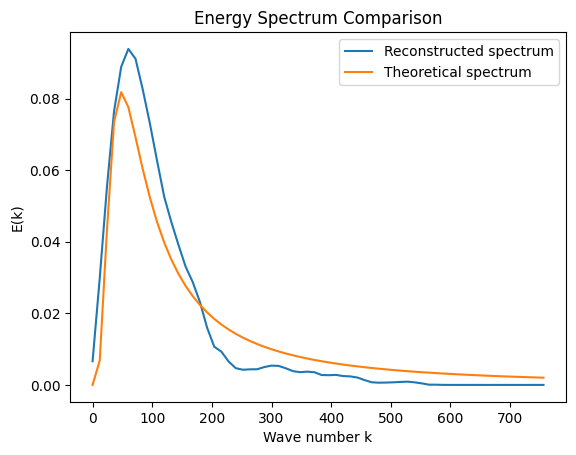
\includegraphics[width=0.55\linewidth]{VelIncrPSIKAPPASIGMA/EnergySpectrum.png}
    \caption{Energy spectrum reconstructed with the learned $(\psi,\kappa,\sigma)$}
  \end{figure}

    \begin{table}
    \centering
    \begin{tabular}{lr}
      \toprule
      \textbf{Direction} & \textbf{Mean} \\
      \midrule
      x & $7.7879E-5$ \\
      y & $5.7016E-5$ \\
      z & -0.0306 \\
      \bottomrule
    \end{tabular}
    \qquad
    \begin{tabular}{lr}
      \toprule
      \textbf{Direction} & \textbf{RMS (expected: 0.222)} \\
      \midrule
      x & 0.00174 \\
      y & 0.00066 \\
      z & 0.88966 \\
      \bottomrule
    \end{tabular}
    \caption{Velocity mean and RMS}
  \end{table}
\end{frame}
\end{comment}


\subsection{Optimizing $(\varphi,\theta,\alpha)$}
\begin{frame}{Results}
  \begin{figure}
    \centering
    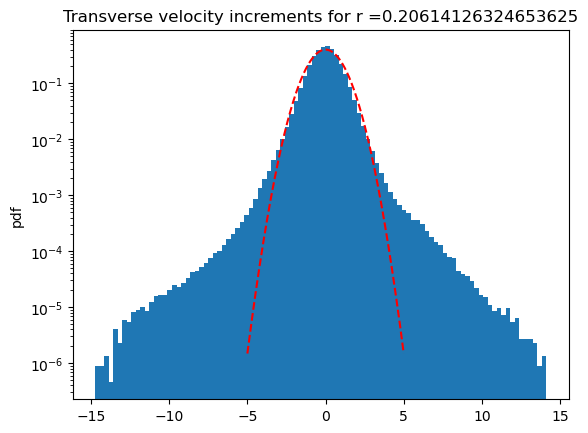
\includegraphics[width=0.47\textwidth]{illustrations/TransVelIncrAngles.png}
    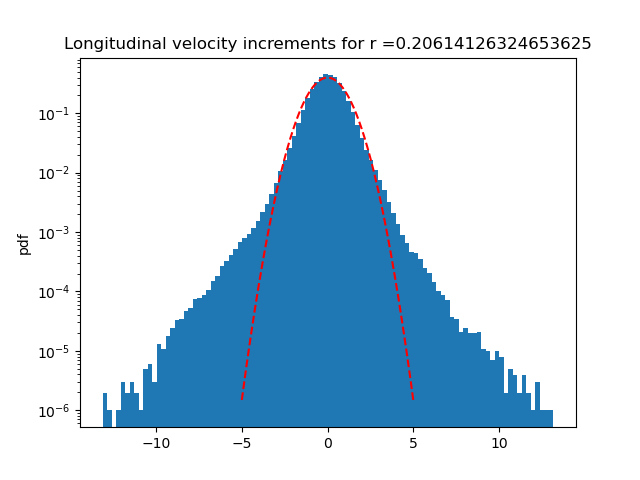
\includegraphics[width=0.49\textwidth]{illustrations/LongVelIncrAngles.png}
    \caption{Velocity increments after learning on $(\varphi,\theta,\alpha)$}
  \end{figure}
\end{frame}

\begin{frame}
  \begin{figure}
    \centering
    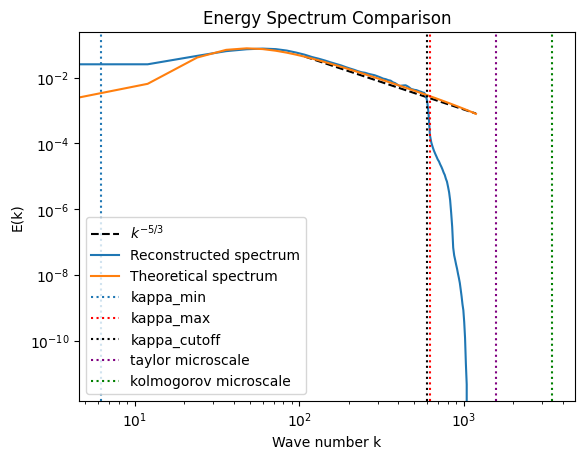
\includegraphics[width=0.49\textwidth]{illustrations/EnergySpectrumTrained.png}
    \caption{Energy spectrum reconstructed with the learned $(\varphi,\theta,\alpha)$}
  \end{figure}

   \begin{table}
    \centering
    \begin{tabular}{lr}
      \toprule
      \textbf{Direction} & \textbf{Mean} \\
      \midrule
      x & 0.002564 \\
      y & -0.00652 \\
      z & -0.00093 \\
      \bottomrule
    \end{tabular}
    \qquad
    \begin{tabular}{lr}
      \toprule
      \textbf{Direction} & \textbf{RMS (expected: 0.222)} \\
      \midrule
      x & 0.12904 \\
      y & 0.31651 \\
      z & 0.11406 \\
      \bottomrule
    \end{tabular}
    \caption{Velocity mean and RMS}
  \end{table}
\end{frame}

\begin{frame}{Vorticity}
  \begin{figure}
    \centering
    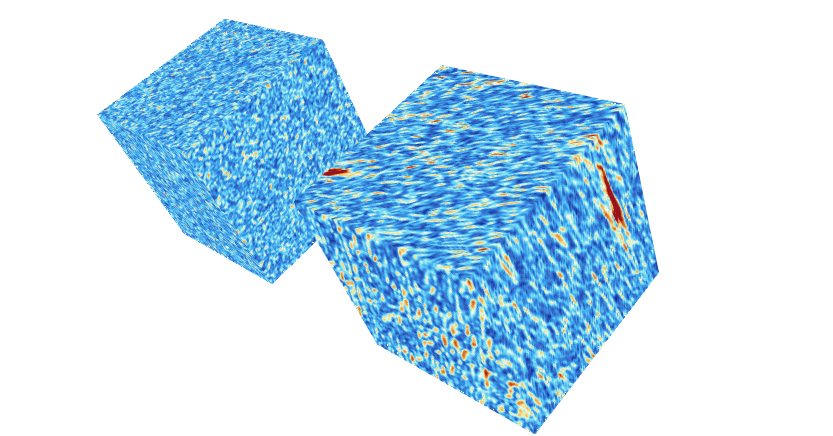
\includegraphics[width=0.65\textwidth]{illustrations/vorticity.png}
    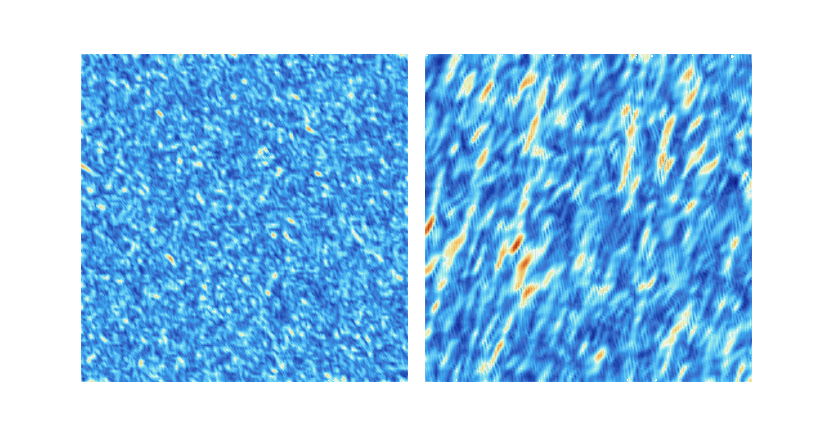
\includegraphics[width=0.49\textwidth]{illustrations/vorticity-cutplane.png}
    \caption{Vorticity field after learning on $(\varphi,\theta,\alpha)$}
  \end{figure}
\end{frame}

\end{document}